\documentclass[a4paper, 10pt, final, garamond]{book}
\usepackage{cours-preambule}

\makeatletter
\renewcommand{\@chapapp}{Devoir surveill\'e -- num\'ero}
\makeatother

\begin{document}
\setcounter{chapter}{6}

\chapter{Commentaires sur le DS n\degree07}

\section{Commentaires généraux}

Vous ne pouvez pas utiliser des exercices indépendants pour obtenir les points
de questions similaires~!

% \begin{figure}[htbp!]
% 	\centering
% 	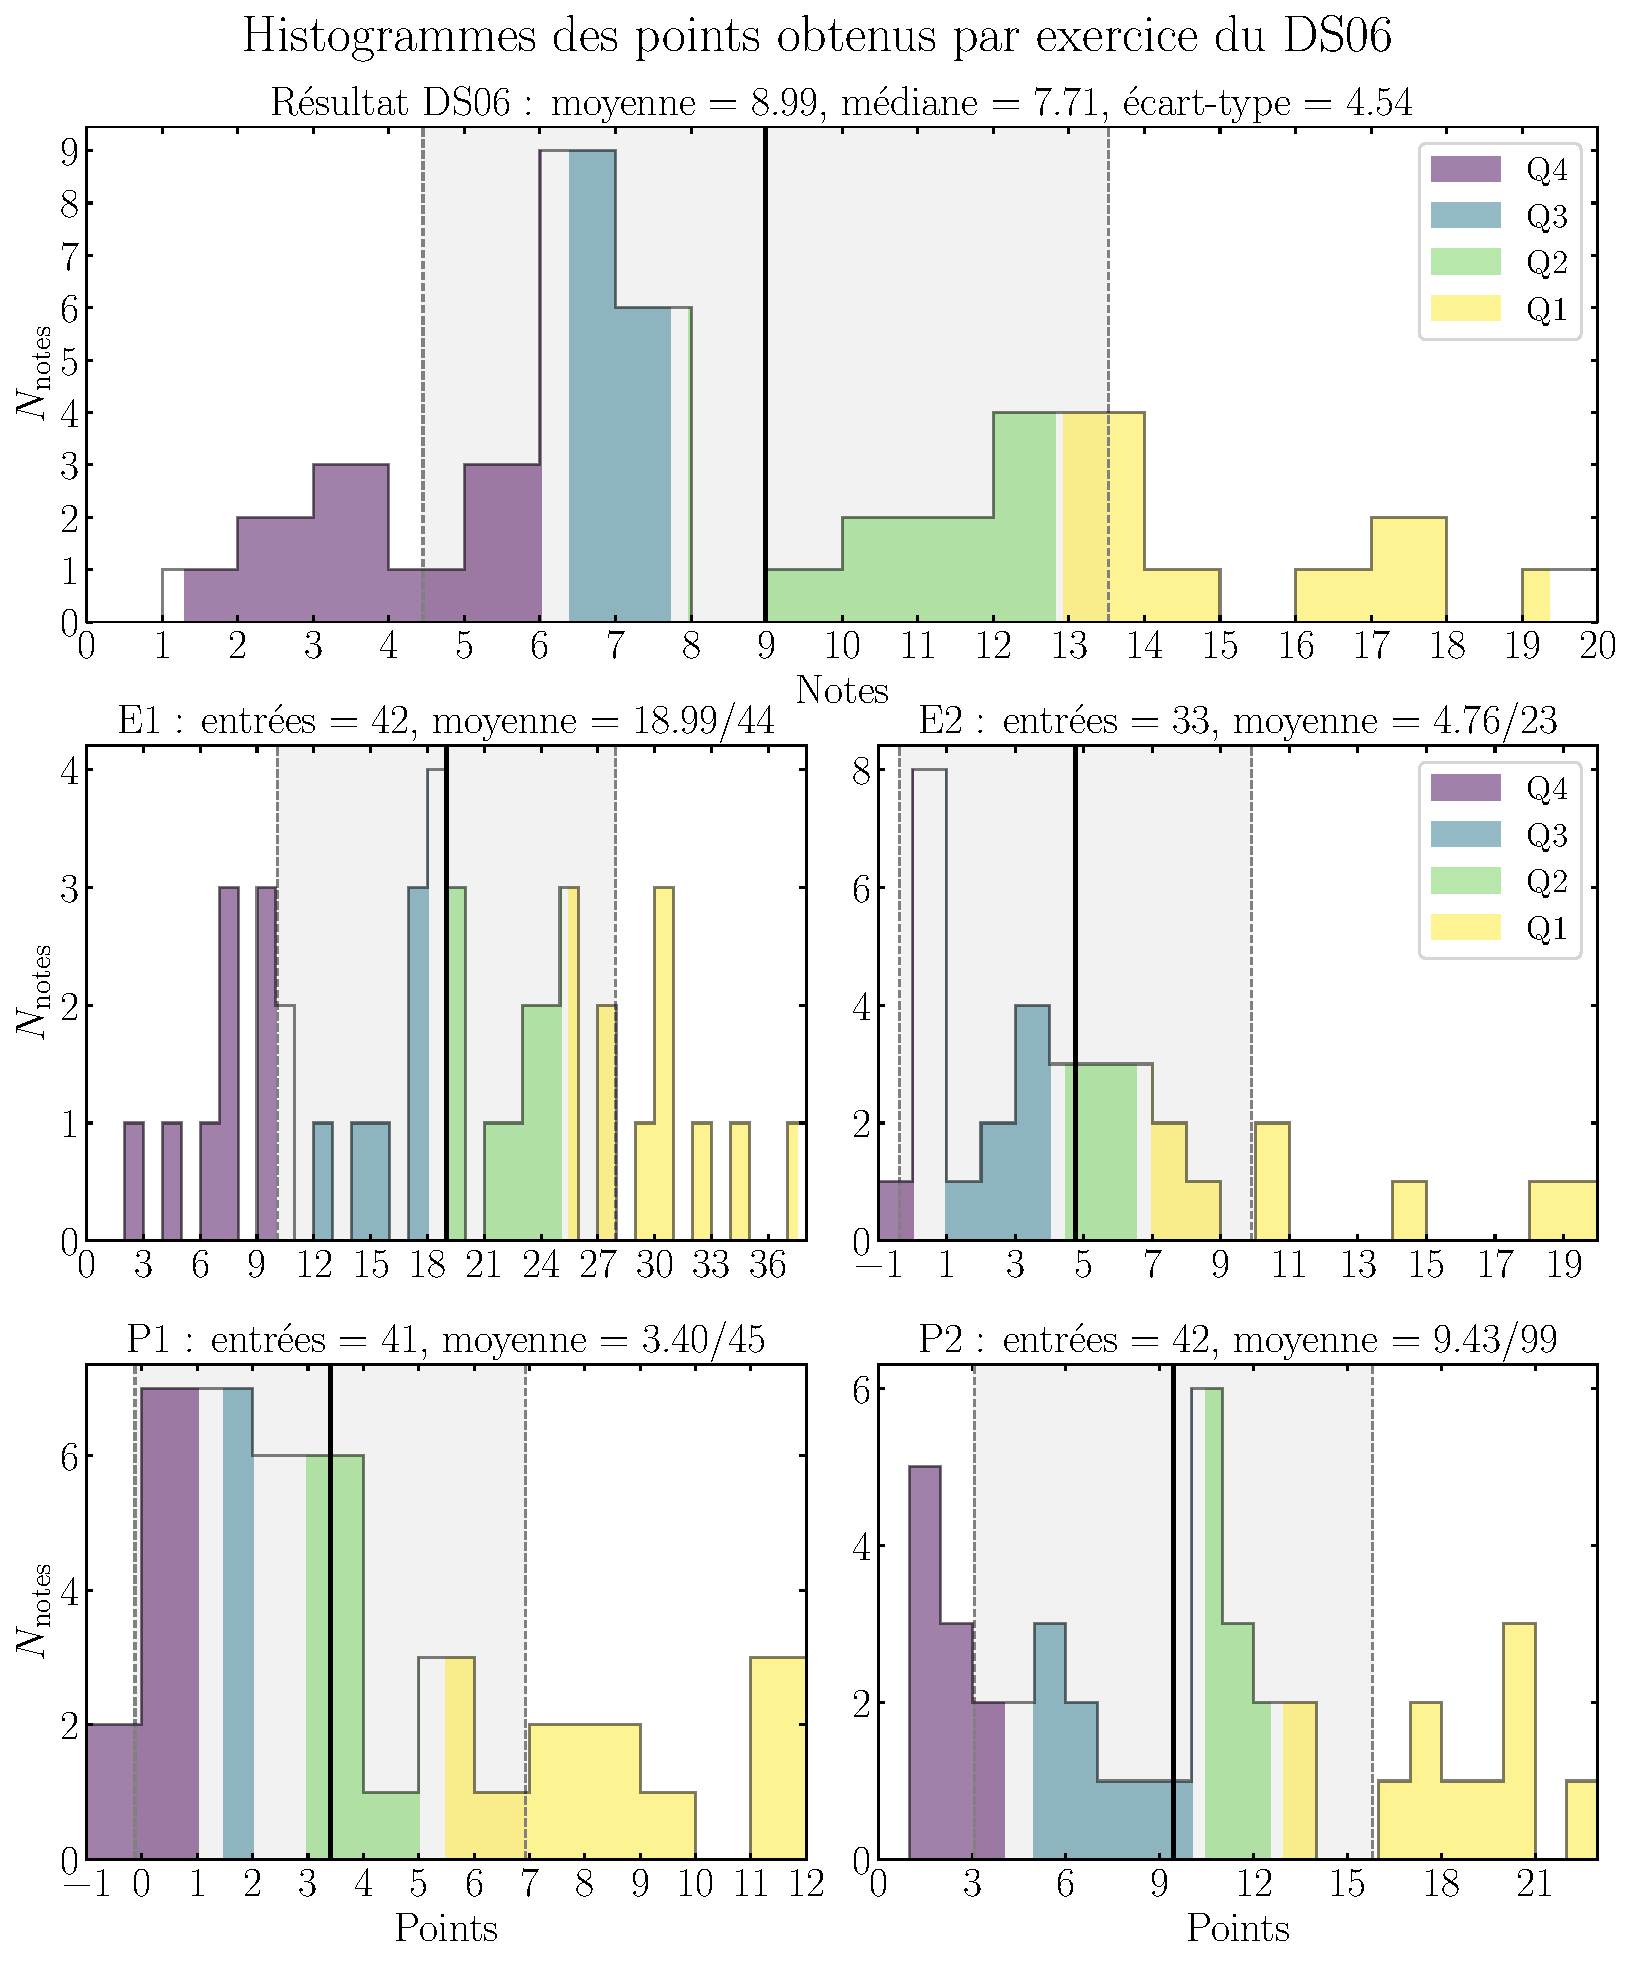
\includegraphics[width=.8\linewidth]{DS06_hist_all}
% \end{figure}

\setcounter{section}{0}
\exercice[20]{Oscillations d'un métronome}
\begin{enumerate}
	\nitem{2}% Q1
	Dans l'idée correcte, mais des formualtions hasardeuses. Beaucoup d'inversions
	alors que, pour rappel, $J$ est l'analogue de $m$ la masse~; donc plus $J$
	augmente plus il est compliqué de faire varier la vitesse du système.
	\nitem{8}% Q2
	Attention à la définition du système, et donc du point d'application ! Si vous
	définissez un poids $\Pf_1 = m\gf$, c'est qu'il s'applique sur le corps de
	massse $m$, pas à un barycentre imaginaire…
	\smallbreak
	Ceci dit, très bien sur les schémas~: forces, bras de levier, moments
	représentés.
	\smallbreak
	Attention à ne pas dire que $d$ du bras de levier vaut $- \ell\sin(\th)$~:
	\textbf{une distance est toujours positive}~! Le signe du moment scalaire
	vient de la projection du moment vecteur sur l'axe de rotation.
	\smallbreak
	Par ailleurs, l'expression $\pm d \norm{\Ff}$ ne vaut \textbf{que pour le
		moment scalaire}~!
	\bigbreak
	$\Gf$ n'est \textbf{pas une force}, c'est un couple donc un \textbf{moment}.
	\smallbreak
	Pas de tension dans un solide (forces intérieures).
	\nitem{2}% Q3
	\nitem{4}% Q4
	\nitem{2}% Q5
	\nitem{2}% Q6
\end{enumerate}

\exercice[47]{Satellite en orbite terrestre}
Des résultats sortis par cœur mais sans analyse de leur signification.
\begin{enumerate}
	\nitem{5}% Q1
	Définitions non connues.
	\nitem{4}% Q2
	Bien, mais il faut définir $\ur$. Énormément de personnes ont oublié le
	$1/r^{\boxed{2}}$~!! Et beaucoup trop ont répondu que la Terre ne subissait
	pas de force de la part du satellite. RIP \textsc{Newton}.
	\nitem{7}% Q3
	\textbf{Ne confondez pas moment cinétique et moment d'une force}~: $\Lcf(\Ff)$
	n'a aucun sens. Pour rappel, $\Lcf(\Sc)$ est la quantité de rotation du
	\textbf{système}, telle que $\Lcf(\Sc) = \OM \wedge \pf$ avec $\pf =
		m\vf(\Mr)$ la quantité de mouvement. Il ne vous viendrait pas à l'esprit de
	parler de la quantité de mouvement d'une force… c'est pareil pour la quantité
	de rotation. Le moment d'une force c'est $\Mcf(\Ff)$.
	\nitem{4}% Q4
	Ne supposez pas que la vitesse est constante sans le montrer (par exemple avec
	\textsc{Frenet} sans $\dv{v}{t}$).
	\nitem{2}% Q5
	RAS.
	\nitem{3}% Q6
	On étudie la rotation d'un satellite \textbf{autour} de la Terre, pas de la
	Terre autour du Soleil, donc $T \neq \SI{365}{jours}$~!
	\nitem{3}% Q7
	\nitem{4}% Q8
	Bravo, vous avez bien intégré le lien entre force conservative et énergie
	potentielle~!
	\smallbreak
	Bien que le produit d'une force centrale avec $\dd{\OM}$ ne donne que la
	composante sur $\ur$, le déplacement élémentaire \textbf{n'est pas
		$\dd{r}\ur$}~!
	\smallbreak
	Intégrez \textbf{avec la constante} puis justifiez sa nullité.
	\nitem{10}% Q9
	Manque souvent de détails. Lisez les questions en entier. Attention au calcul
	de $v^2$~: j'ai vu d'innombrables $v^2 = (\rp + r\rp)^2$~! Soit avec des
	bonnes réponses ensuite, soit pas, mais il faut savoir calculer une norme
	corretement.
	\nitem{5}% Q10
\end{enumerate}

\setcounter{section}{0}
\prblm[48]{Rotation d'un œuf dur}
\begin{enumerate}
	\nitem{2}% Q1
	Mauvaises interprétations, ou explications trop verbeuses.
	\nitem{2}% Q2
	Depuis que je vous ai dit de faire attention au signe de l'énergie
	potentielle, vous pensez qu'il y a toujours un signe $«~-~»$… l'énergie
	potentielle \textbf{augmente avec l'altitude}, peu importe le système de
	coordonnées~!
	\nitem{3}% Q3
	Erreur de calcul courante avec le $\frac{1}{5} - \frac{1}{10}$. De plus, il
	faut voir la simplification des identités remarquables $(b-a)/(b^2-a^2)$.
	\nitem{2}% Q4
	\nitem{3}% Q5
	\nitem{7}% Q6
	\nitem{4}% Q7
	\nitem{5}% Q8
	\nitem{4}% Q9
\end{enumerate}

\prblm[64]{Satellites de télécommunication}
\begin{enumerate}
	\nitem{9}% Q1
	Établir = \xul{démontrer}. $h$ est l'altitude, donc \textbf{pas} la distance
	entre le centre de la Terre et le satellite.
	\nitem{2}% Q2
	Ne confondez pas l'énergie potentielle de pesanteur et l'énergie potentielle
	gravitationnelle~!
	\nitem{5}% Q3
	\nitem{3}% Q4
	\nitem{3}% Q5
	\nitem{7}% Q6
	Ne confondez pas unité ($[\ell] = \si{m}$) et dimension ($\dim{\ell} = L$).
	\nitem{5}% Q7
	\nitem{8}% Q8
	\nitem{7}% Q9
	\nitem{2}% Q10
	\nitem{5}% Q11
	\nitem{8}% Q12
\end{enumerate}

\end{document}
